\documentclass[11pt,a4paper]{article}
\usepackage[margin=20mm,headheight=15pt]{geometry}
\usepackage[T1]{fontenc}
\usepackage[utf8]{inputenc}
\usepackage{lmodern,microtype,graphicx,booktabs,array,tabularx,amsmath,xcolor,fancyhdr,enumitem}
\usepackage[colorlinks=true,urlcolor=blue!55!black,linkcolor=blue!55!black]{hyperref}
\definecolor{ink}{RGB}{23,54,75}
\definecolor{muted}{RGB}{70,81,92}
\pagestyle{fancy}\fancyhf{}\lhead{\small Diabetes 130-US Hospitals}\rhead{\small Supervised Learning \& Model Engineering}\cfoot{\thepage}
\setlength{\emergencystretch}{3em}
\setlength{\parindent}{0pt}\setlength{\parskip}{6pt}
\setlist[itemize]{topsep=2pt,itemsep=2pt,leftmargin=16pt}
\renewcommand{\arraystretch}{1.16}
\newcommand{\pageheading}[2]{\section*{\color{ink}#1. #2}}
\newcommand{\fig}[3]{\begin{center}\includegraphics[width=#2\linewidth]{images/#1}\par{\small\color{muted}#3}\end{center}}
\newcommand{\nextpage}{\clearpage}
\begin{document}
{\LARGE\bfseries\color{ink} Predicting recorded hospital readmission}\par
{\large Diabetes 130-US Hospitals, OpenML dataset 4541}\par
Matis Douay \quad Driss Haddadi \quad Rayan Faher Bonne\\
MSA-DATB09-04 \quad Ilana Sebag \quad Fall 2026\\
Repository: \url{https://github.com/matisdy/diabetes-submission}

\pageheading{1}{Problem framing and exploratory analysis}
We study a tabular binary classification problem using 101,766 encounters from 71,518 patients in the Diabetes 130-US Hospitals dataset. The records cover 1999--2008. Each row describes a hospital stay, rather than a distinct person. Of the patients, 16,773 have several stays, accounting for 47,021 encounters. This repeated-observation structure determines our evaluation design: all stays from one patient must remain in the same partition.

The original target has three categories: \texttt{NO} (54,864 encounters), \texttt{>30} (35,545) and \texttt{<30} (11,357). We map both readmission categories to 1 and \texttt{NO} to 0, obtaining 46,902 positives (46.09\%). Our problem is therefore \emph{recorded readmission at any delay}, rather than specifically readmission within 30 days. This aggregate question provides a broad illustration of readmission patterns, but sacrifices the distinction between early and later returns. \texttt{NO} means that a readmission was not recorded in this dataset; it does not establish that none occurred elsewhere.

Prediction is situated at discharge, when stay duration, procedures, medications and discharge disposition are available. The exercise could inform investigation of follow-up allocation, but we do not estimate clinical benefit, intervention costs or prospective reliability. It is a supervised-learning proof of concept.

\begin{center}\begin{tabular}{lr}\toprule
Exploratory observation & Value\\\midrule
Raw predictor columns & 49\\
Target missing values / duplicated rows & 0 / 0\\
Mean / median stay duration & 4.40 / 4 days\\
Stay-duration range & 1--14 days\\
Mean laboratory procedures per encounter & 43.10\\\bottomrule
\end{tabular}\end{center}
We retain the encounter population used in the final notebook. This includes stays ending in death: discharge disposition 11 is a strongly predictive negative indicator. Such encounters are not candidates for post-discharge follow-up. Their inclusion makes the classification task broader than a follow-up service and can increase apparent usefulness by identifying structurally negative cases. We retain this limitation rather than revise the population after observing test results.

\textbf{Evidence scope.} The numerical results and figures in this report come from the frozen final notebook and its retained Optuna/fairness artifacts. Development CV results, validation diagnostics and final test results are distinguished throughout. Packaging the implementation does not constitute a new model search.

\nextpage
\pageheading{2}{Data preparation and feature engineering}
\textbf{Missingness.} Several unknown entries are represented by \texttt{?}, while gender also contains \texttt{Unknown/Invalid}. These markers are normalized before modelling. The original notebook also normalizes \texttt{None} in biological-test columns before removing those columns. Here \texttt{None} means that a test was not performed, so it is informative absence rather than an unknown measurement.

\begin{center}\begin{tabular}{lrp{72mm}}\toprule
Removed variable & Apparent missingness & Interpretation and limitation\\\midrule
\texttt{weight} & 96.86\% & Mostly unknown.\\
\texttt{max\_glu\_serum} & 94.75\% & Includes tests not performed.\\
\texttt{A1Cresult} & 83.28\% & Includes tests not performed.\\
\texttt{medical\_specialty} & 49.08\% & Unknown specialty information.\\
\texttt{payer\_code} & 39.56\% & Unknown payer information.\\\bottomrule
\end{tabular}\end{center}
We use this reduced predictor set to keep the proof of concept manageable. We have not established through ablation that these variables are uninformative, nor that imputation would necessarily be invalid. In particular, excluding the test columns discards information about test ordering. This is a modelling limitation, not an evidence-based demonstration that removal improves prediction.

Unknown diagnosis codes are filled with the explicit category \texttt{Unknown}. Encounter and patient identifiers are removed from predictors; the patient identifier remains available separately for grouping. Diagnosis codes, admission codes and discharge codes are treated as categories, since their numeric labels do not express meaningful distances.

\textbf{Two justified derived features.} We calculate these row-wise without estimating population parameters:
\begin{align*}
\texttt{previous\_visits} &= \texttt{number\_outpatient}+\texttt{number\_emergency}+\texttt{number\_inpatient},\\
\texttt{lab\_procedures\_per\_day} &= \frac{\texttt{num\_lab\_procedures}}{\texttt{time\_in\_hospital}}.
\end{align*}
The first summarizes healthcare utilization during the preceding year. The second describes average laboratory-testing intensity during the stay. Stay duration is at least one day in these data, so this ratio has no zero denominator. Both are available at the stated discharge prediction time. They complement, rather than replace, their source variables; their incremental benefit was not separately measured.

\textbf{Learned preprocessing.} Ten numerical columns receive median imputation and standard scaling. Categorical columns receive constant \texttt{Unknown} imputation and one-hot encoding with unseen categories ignored. For CatBoost, the categorical values remain categorical and are passed by column name, while numerical values receive median imputation. This preserves the library's native categorical handling.

The Python implementation joins fixed preparation, learned preprocessing and the estimator in one scikit-learn \texttt{Pipeline}. Its first step, \texttt{PrepareEncounters}, applies the same marker cleaning, identifier/column removal and two feature calculations as the notebook. It learns no parameters. The following steps fit imputation, scaling and encoding within each CV training fold. The saved Pipeline therefore accepts all 49 raw predictor columns directly and reuses the same sequence during prediction.

\nextpage
\pageheading{3}{Evaluation design and imbalance strategy}
\textbf{Patient-separated outer test.} We use the first split of shuffled five-fold \texttt{GroupKFold}, with seed 42 and patient number as the group. Approximately 80\% of encounters form the development set and 20\% form the held-out test set. The proportions of encounters are approximate because groups contain different numbers of stays.

\begin{center}\begin{tabular}{lrr}\toprule
Partition & Encounters & Role\\\midrule
Development & 81,613 & Model comparison and tuning\\
Final test & 20,153 & Frozen before/after evaluation\\\midrule
Final fitting subset & 65,146 & Fit final base model\\
Development validation subset & 16,467 & Diagnostics and mitigation\\\bottomrule
\end{tabular}\end{center}
There is no patient overlap between development and test. The inner five-fold CV also groups by patient and uses the same seed and folds for every compared model. The final fitting/validation split is again taken from this grouped CV: these two subsets have no patient overlap. Patient identifiers are retained for grouping, then removed by the first Pipeline step before learned preprocessing and model fitting.

The preprocessing is part of each estimator passed to \texttt{cross\_validate}. Imputation values, scaling statistics and encoded categories are therefore learned from the training fold, rather than estimated once using its validation data. This is the main protection against learned-preprocessing leakage emphasized in Session 5 [2]. The fixed row-wise arithmetic does not learn from the held-out targets or distributions.

\textbf{Selection and diagnostics are different uses of development data.} Tuning sees all development patients across folds. We subsequently fit the retained configuration on 65,146 stays and use the 16,467-stay validation subset for probability diagnostics and threshold mitigation. This subset did participate in hyperparameter selection, so its diagnostic estimates are not entirely independent of selection. The final test was not used for fitting preprocessing, tuning the base classifier or learning mitigation rules.

We do not refit the base model on the whole development set after fitting the mitigation. Its validation predictions define the relationship used to learn post-processing rules; changing the underlying estimator would change that relationship. The test evaluation concerns this fixed fitting-subset model and its associated post-processor.

\textbf{Moderate class imbalance.} Positives represent 46.27\% of development stays. We preserve the observed distribution and avoid over- or undersampling. Both boosting searches include optional class weighting. The selected LightGBM configuration is unweighted; the selected CatBoost configuration uses \texttt{Balanced}. Other parameters vary between trials, so these selections do not isolate a causal effect of weighting. SMOTE is optional in Session 6 [3] and is not justified merely by a small deviation from 50/50.

Accuracy, precision, recall, F1 and ROC-AUC are reported consistently. Thresholded metrics use the usual 0.5 rule until mitigation; ROC-AUC summarizes ranking across thresholds. We do not assign unequal clinical error costs because none were measured. There is no temporal or external-hospital holdout, so patient separation establishes a limited generalization claim rather than future or cross-site validity.

\nextpage
\pageheading{4}{Modelling progression}
We compare four approaches under the same five-fold patient-grouped development protocol. Logistic Regression provides a linear baseline for associations between the predictors and target. Random Forest tests nonlinear trees and interactions through averaging. LightGBM tests sequential gradient-boosted trees with efficient training. CatBoost is relevant to the many categorical variables, particularly diagnosis codes.

\begin{center}\small\begin{tabular}{lrrrrr}\toprule
Initial model & Accuracy & Precision & Recall & F1 & ROC-AUC\\\midrule
Logistic Regression & .6375 & .6273 & .5332 & .5764 & .6909\\
Random Forest & .6400 & .6332 & .5276 & .5756 & .6917\\
LightGBM & .6457 & .6332 & .5572 & .5927 & .7023\\
CatBoost & .6494 & .6350 & .5698 & .6005 & .7073\\\bottomrule
\end{tabular}\end{center}
\textit{All values are mean development-CV scores from the saved notebook, not final test scores.}

\textbf{What each step buys.} The Random Forest AUC is only about 0.0008 above the logistic baseline, and its recall and F1 are slightly lower. More expressive modelling alone therefore does not guarantee a meaningful gain. The two boosting methods achieve clearer improvements in discrimination and recall, with similar precision. Relative to Logistic Regression, CatBoost gains about 0.0164 AUC and 0.0241 F1. We retain the two boosting candidates for tuning rather than spend further search budget on all four initial estimators.

\begin{center}\begin{tabular}{lrr}\toprule
Initial model & Mean fit time per fold & Mean score time per fold\\\midrule
Logistic Regression & 2.17 s & 0.15 s\\
Random Forest & 61.23 s & 1.14 s\\
LightGBM & 1.04 s & 0.20 s\\
CatBoost & 15.85 s & 0.18 s\\\bottomrule
\end{tabular}\end{center}
These are recorded timings from these particular notebook runs. They depend on hardware, library settings, data representation and current estimator sizes. They are not controlled latency benchmarks and do not imply that a slower search necessarily produces a slower prediction service.

The default models are Logistic Regression with \texttt{max\_iter=1000}, a seeded Random Forest, a seeded LightGBM and a CatBoost with 300 iterations and native categorical columns. No target-derived feature is added. Model randomness and grouped CV use seed 42.

\textbf{Interpretation of small differences.} The same folds improve comparability, but five correlated fold estimates do not establish statistical significance. The best two models remain close in absolute AUC. Their development scores have also been used for model selection, so they should not be described as an unbiased final estimate. The held-out evaluation later in the report addresses that role for the selected pipeline.

The comparison satisfies the minimum of three model families while retaining a simple baseline. We keep the progression and its imperfect gains visible, instead of presenting only the best boosting score. A more exhaustive study could compare feature ablations and cost-sensitive operating points, but these are not additional experiments performed in this submission.

\nextpage
\pageheading{5}{Optuna search, tracking and model choice}
Each retained candidate receives 50 Optuna trials. A seeded TPE sampler maximizes mean ROC-AUC from the same five-fold grouped CV, with preprocessing fitted inside every fold. We store trials in the SQLite file \texttt{optuna\_results.db}; reload-by-name and a remaining-trials guard prevent a normal rerun from adding another 50 trials to a completed study.

\begin{center}\small\begin{tabular}{lp{53mm}p{53mm}}\toprule
 & LightGBM & CatBoost\\\midrule
Search space & 100--500 trees (step 100); learning rate .01--.2; leaves 15--127; minimum child samples 20--100 (step 20); weighting None/balanced & 100--500 iterations (step 100); learning rate .01--.2; depth 4--8; weighting None/Balanced\\
Best parameters & 400 trees; rate .020617; 71 leaves; minimum child samples 100; no class weighting & 500 iterations; rate .052303; depth 8; Balanced\\
Best mean CV AUC & .705331 & .708707\\\bottomrule
\end{tabular}\end{center}
\fig{cell-106-0.png}{.64}{Recorded LightGBM optimization history, extracted from the final notebook.}
Tuning improves LightGBM from .7023 to .7053 and CatBoost from .7073 to .7087. These are modest development improvements. CatBoost scores higher in all five folds of the best-configuration comparison, with a mean advantage of approximately .0034 AUC. We retain LightGBM as a computational trade-off, accepting this observed performance difference for its lower training/search cost in the recorded runs. We do not claim equal performance or superior prediction latency.

The SQLite histories and exported CSVs preserve sampled parameters, trial values and states, timestamps, fold-level metrics and fitting/scoring times. Optimization-history plots are retained as artifacts. Four initial model families are compared under the same CV protocol; the two strongest boosting candidates then receive the tuning budget. The retained histories correspond to those two candidate searches. The trial guard is valid only for an unchanged dataset, target, preprocessing and folds.

\nextpage
\pageheading{6}{Global explainability}
We fit the selected LightGBM configuration on the final fitting subset and use this exact estimator for explanation, calibration and test evaluation. Its gain importance ranks transformed columns by the total training-objective improvement associated with their splits. Gain is a model-internal measure, not a causal effect or an independent measure of future usefulness.

\fig{cell-113-0.png}{.78}{Top ten gain importances of the fixed final LightGBM.}
Previous utilization dominates: \texttt{previous\_visits} and \texttt{number\_inpatient} have the largest gains. This is consistent with the model using prior healthcare use to identify patients more likely to have another recorded encounter. Both source counts and their aggregate are retained, so their importances may share related information. Their individual ranks should not be interpreted as independent effects.

The discharge-disposition indicator for code 11 ranks third. Its negative effect for affected encounters reflects the death-related cohort limitation identified in the problem framing. Strong prediction can partly reflect outcome structure rather than actionable variation among patients eligible for follow-up. This feature is available at the stated discharge time; the concern is the interpretation of the cohort, rather than automatically a temporal data leak.

Laboratory counts, diagnosis counts, medications, testing intensity and stay duration also appear. They plausibly describe severity and care patterns at discharge, but the model does not establish the medical mechanism of any association. The high rank of the engineered visit aggregate and the appearance of testing intensity confirm that both added features are actually used by the fitted model. No ablation establishes their isolated performance contribution.

\textbf{Limits of importance.} Diagnosis and category columns are represented by many one-hot indicators. Their separate gains are not directly comparable to an aggregated original variable, and correlated predictors can divide importance. Gain should therefore be read together with SHAP and domain context, as emphasized in Session 8 [5]. We do not translate a high gain into a recommendation to change treatment.

\nextpage
\pageheading{7}{SHAP and individual predictions}
\fig{cell-115-1.png}{.72}{SHAP summary for 300 seeded development stays; horizontal values are log-odds contributions.}
We use \texttt{TreeExplainer} on the final model with \texttt{model\_output="raw"}. The sample comes from the development set and mixes fitting and validation observations; it is descriptive rather than a separate generalization assessment. The fitted preprocessing is reused to obtain exactly the transformed columns expected by the model. Colour encodes the transformed feature value.

For an observation, the SHAP baseline and all feature contributions reconstruct the raw score. Applying the logistic link converts that score into a probability. A contribution of .2 log-odds does \emph{not} mean a 20-percentage-point risk increase. The notebook checks additivity for each of the three examples below, and all checks return true.

\begin{center}\small\begin{tabular}{lrp{104mm}}\toprule
Stay index & Probability & Main local interpretation\\\midrule
39397 & .60575 & Diagnosis indicator 491 contributes +.176 and admission source 7 +.162; inpatient history contributes -.213, while the aggregate of previous visits contributes +.122.\\
66309 & .23158 & Previous visits (-.301), inpatient visits (-.161) and stay duration (-.094) lower the raw score; admission source 7 contributes +.089.\\
42168 & .53133 & Diagnosis indicator 428 in the second diagnosis column contributes +.187 and diagnosis count +.102, offsetting previous visits (-.224) and inpatient visits (-.103).\\\bottomrule
\end{tabular}\end{center}
These indices identify rows in the analysis, not patient identifiers used as model inputs. The displayed numerical values in the notebook are standardized, whereas category indicators are encoded values. Interpreting their magnitudes requires respecting this representation.

SHAP explains how this fitted predictor allocates contributions relative to its baseline. It does not identify what would happen under an intervention, prove a clinical mechanism, or make changing an input a valid treatment strategy. The combined global and local views make the model auditable while preserving these limits.

\nextpage
\pageheading{8}{Probability calibration diagnostics}
\begin{center}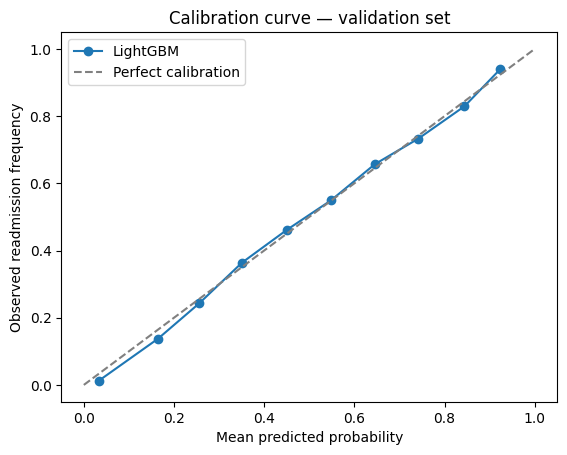
\includegraphics[width=.49\linewidth]{images/cell-122-0.png}\hfill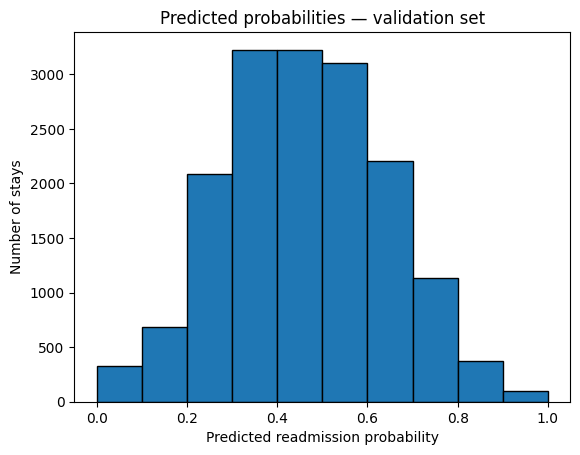
\includegraphics[width=.49\linewidth]{images/cell-125-0.png}\par{\small\color{muted}Validation reliability diagram and predicted-probability distribution, with ten equal-width bins.}\end{center}
Ranking and calibration answer different questions: ROC-AUC concerns ordering, while calibration concerns whether predicted probabilities agree with observed frequencies [4]. We assess the fixed final pipeline on the 16,467-stay development validation subset. No recalibration map is fitted.

The Brier score is the average squared difference between the probability and binary outcome:
\[ \mathrm{Brier}=\frac{1}{n}\sum_{i=1}^{n}(p_i-y_i)^2=0.215525. \]
It measures overall probability quality, combining calibration and discrimination properties; it is not a pure calibration statistic. The expected calibration error (ECE) averages the absolute difference between mean probability and observed frequency in each occupied bin, weighted by its fraction of observations:
\[ \mathrm{ECE}=\sum_b\frac{n_b}{n}\,\left|\overline p_b-\overline y_b\right|=0.010763. \]

The reliability curve is broadly near the diagonal. It shows some overestimation in lower predicted-risk bins, with deviations elsewhere varying in direction. We therefore do not identify a strong uniform overconfidence or underconfidence pattern. An ECE near .01 is encouraging at this binning resolution, but can conceal local or subgroup errors. It depends on bin choices and is not a guarantee of trustworthy individual probabilities.

The accompanying histogram is essential: bins with few observations can have unstable observed rates. Extreme probabilities are sparse, so a visually large deviation there should not be treated as equally well estimated as a deviation in a populated central bin. No uncertainty bands or segment-specific calibration estimates are provided.

We retain the model's original probabilities for this proof of concept. The diagnostics support approximate aggregate calibration on this validation population; they do not establish readiness for automated clinical decisions. The subset already participated in hyperparameter selection, so these diagnostics are not fully independent of model selection. A future use would require prospective or external validation, checking population and prevalence changes, defining error costs and evaluating important subgroups before deciding whether recalibration is needed.

\nextpage
\pageheading{9}{Fairness audit and mitigation}
We audit race groups, with an explicit \texttt{Unknown} category. Our fairness definition is equalized odds: similar true-positive rates (TPR) and false-positive rates (FPR) across groups. In an illustrative follow-up allocation setting, false negatives would be unflagged readmitted stays and false positives would consume follow-up resources without a recorded readmission. We examine both errors rather than equalizing only the number of alerts. Actual intervention costs were not estimated.

We compute each rate from group confusion matrices. The reported equalized-odds gap is the larger of the max-minus-min TPR and FPR gaps. On development validation at threshold .5, it is .4187. Small groups, particularly 95 Asian validation encounters, make estimates uncertain. This number is a validation diagnostic, not the final test gap.

We fit Fairlearn \texttt{ThresholdOptimizer} on validation data, with a prefitted fixed pipeline, an equalized-odds constraint and an accuracy objective. The method learns race-dependent decision rules, which can involve randomization. The fixed seed makes the reported realization reproducible. It changes binary decisions while retaining the original probability scores.

\begin{center}\small\begin{tabular}{lrrrr}\toprule
Final test & Accuracy & Precision & Recall & F1\\\midrule
Before mitigation & .6484 & .6229 & .5694 & .5950\\
After mitigation & .6425 & .6072 & .5993 & .6032\\\bottomrule
\end{tabular}\qquad
\begin{tabular}{lrrr}\toprule
Gap & TPR & FPR & EO\\\midrule
Before & .2080 & .2010 & .2080\\
After & .1109 & .0664 & .1109\\\bottomrule
\end{tabular}\end{center}
The final test comprises 20,153 encounters. Its unchanged base-score ROC-AUC is \textbf{.706915}; we do not compute an AUC from the randomized binary mitigation output and present it as probability quality. Mitigation lowers the EO gap by about .0971, but does not fully achieve equalized odds on unseen patients.

\begin{center}\small\begin{tabular}{lrrrrr}\toprule
Test group & Stays & TPR before & TPR after & FPR before & FPR after\\\midrule
AfricanAmerican & 3,847 & .558 & .606 & .292 & .335\\
Asian & 125 & .423 & .615 & .151 & .370\\
Caucasian & 15,089 & .579 & .601 & .296 & .316\\
Hispanic & 393 & .542 & .542 & .244 & .319\\
Other & 289 & .477 & .505 & .174 & .382\\
Unknown & 410 & .371 & .578 & .095 & .347\\\bottomrule
\end{tabular}\end{center}
FPR rises in every group: reduced disparities come with more false alarms. The Other group has the lowest mitigated recall (.505), and Unknown the lowest mitigated precision (.396). Small samples limit interpretation. Race is required at prediction time for this procedure. Equalized odds does not imply equal precision, selection rates or calibration, and these results do not prove that the system is fair in all senses [6].

\nextpage
\pageheading{10}{Engineering delivery, limitations and conclusion}
\textbf{From notebook to executable implementation.} The main deliverable consists of organized Python scripts, persistent Optuna studies, selected evaluation artifacts and a local prediction endpoint. The repository also includes the dataset snapshot and schema, a saved model bundle, this LaTeX report and the presentation. The original notebook is retained by the group as source evidence. The README specifies installation, reproduction and service commands. The endpoint serves recorded-readmission probabilities and decisions as a coursework demonstration.

Raw encounters are passed directly to the fitted Pipeline: fixed preparation, derived features, imputation, category encoding and scaling precede the model. The fixed transformer preserves the notebook's calculations and does not add a new model or feature. The fitted base Pipeline and mitigation rules belong together. The probability belongs to the base model, while the optional mitigated decision uses the supplied race group; an optional seed reproduces a particular randomized output (seed 42 for the reported evaluation). Those two outputs answer distinct questions and should not be conflated. Engineering the input path does not change the statistical problem or authorize new tuning on the already-observed test set.

\textbf{Main findings.} Boosting improves on the logistic baseline, while Random Forest adds little under the initial settings. Tuning yields modest additional gains. CatBoost has the highest development AUC, but LightGBM is retained for a computational trade-off. The fixed final LightGBM reaches .7069 test ROC-AUC. Its validation probabilities are approximately calibrated at aggregate bin level. Equalized-odds post-processing reduces the test error-rate gap from .2080 to .1109, accompanied by higher recall, lower accuracy and precision, and higher false-positive rates.

\textbf{Limits and next validation.} The binary target merges two readmission delays. Negative labels reflect dataset recording, not guaranteed lifetime absence of readmission. The full cohort includes deaths and may reward structurally easy negatives. The historical dataset and patient-random split cannot establish future or hospital-transfer performance. The validation subset was used in selection, and calibration lacks confidence intervals and subgroup diagnostics. SHAP is descriptive and uses a mixed development sample. The two tuned candidates were selected after comparing four families. The unified raw-input Pipeline changes how preprocessing is packaged, while preserving the statistical protocol.

A next study should predefine a deployment-eligible cohort and time horizon, obtain genuinely external or later data, and specify intervention costs with stakeholders. Such changes require a new evaluation protocol. The present project demonstrates the course workflow and its trade-offs; it does not validate a clinical service.

\textbf{References and source evidence.}\par
{\small
\mbox{[1]} Ilana Sebag. \emph{Final Project Instructions}, MSA-DATB09-04, pp. 1--3.\\
\mbox{[2]} Ilana Sebag. \emph{Session 5: Pipelines, hyperparameter search, and nested cross-validation}, Fall 2026.\\
\mbox{[3]} Ilana Sebag. \emph{Session 6}, class imbalance, metrics, weights and resampling.\\
\mbox{[4]} Ilana Sebag. \emph{Session 7}, calibration diagnostics and probability trust.\\
\mbox{[5]} Ilana Sebag. \emph{Session 8}, diagnostics and SHAP explanations.\\
\mbox{[6]} Ilana Sebag. \emph{Session 9}, fairness definitions and mitigation trade-offs.\\
\mbox{[7]} OpenML dataset 4541, \emph{Diabetes 130-US Hospitals}. Loaded with \texttt{fetch\_openml(data\_id=4541, as\_frame=True)}.\\
\mbox{[8]} Group final \texttt{diabetes.ipynb}; retained SQLite studies and fairness CSVs. Figure numbers in the artifact filenames identify notebook source cells.
}

\nextpage
\appendix
\section*{Appendix A. Contribution and AI-use declaration}
\textbf{Contribution statement -- individual attribution requires group confirmation.}

The named group members are Matis Douay, Driss Haddadi and Rayan Faher Bonne. The final notebook was supplied as the group's existing work. Read-only local Git history provides the provisional attribution below. Commit authorship records changes, but does not capture all collaborative work or establish individual understanding. The group must confirm this account before submission, particularly the account-to-name association for Rayan.

\begin{center}\begin{tabularx}{\linewidth}{lX}\toprule
Member & Individual contribution declaration\\\midrule
Matis Douay & Account \texttt{matisdy}: completion of the remaining notebook (\texttt{cc6a1b8}, 20 October 2026); delivery coordination was directly observed in the preparation request.\\
Driss Haddadi & Author \texttt{Driss}: EDA, feature engineering, imbalance handling, README and dependencies (\texttt{8d0bd88}, 19 October; \texttt{719fbc4}, 20 October 2026).\\
Rayan Faher Bonne & Modelling progression, Pipeline and tuning (\texttt{87729fe}, 20 October 2026), recorded under \texttt{ayama0418} on branch \texttt{rayan}; mapping this account to Rayan is inferred and requires confirmation.\\\bottomrule
\end{tabularx}\end{center}
\textbf{AI assistance.} AI provided some guidance on the technical parts of the project, particularly requirements 4 (modelling), 8 (explainability) and 9 (calibration). It also helped structure the delivery repository and draft this report.

\textbf{Submission actions retained by the group.} Confirm and replace the contribution table with the real division of work; verify the AI-use declaration reflects the full history; review the source and PDF; verify the repository URL. The submission repository contains the Python implementation and report sources; the group's original working history remains the evidence for the provisional attribution above. All members should rehearse both presentation and questions.

\textbf{Artifact provenance.} Report figures are extracted from saved outputs of the frozen final notebook, not regenerated experiments. Original source-cell filenames are retained under \texttt{images/}. The source notebook remains unchanged. The implementation reconstructs the same fixed evaluation and checks key metrics against the frozen results.
\end{document}
